\chapter{Grundlagen}\label{kap:grundlagen}
\section{Softcore-Prozessoren}\label{kap:softcoreprozessoren}

Ein SoftCore (engl. „Software-Kern“) ist ein Prozessor, Mikrocontroller oder ein Signalprozessor, welcher als virtuelle Einheit in einem \ac{fpga} oder \ac{asic} integriert wird.
Dies bietet die Möglichkeit einem digitalen Schaltungsdesign jeden beliebigen Prozessor hinzuzufügen.\\
Umgesetzt wird dieser Vorgang im \ac{fpga} durch reine Anwenderlogik,
welche dementsprechend konfiguriert werden muss.\\
Das typische Anwendungsgebiet eines SoftCores ist die Lösung von komplizierten Aufgaben, mit denen klassische „State Machines“ überfordert sind oder die Effektivität
 nicht mehr gegeben ist. Somit werden SoftCores oftmals nachträglich in bestehende Designs eingefügt, wenn deren Umfang sich extrem vergrößert hat.\cite{softcore}\\

\subsection{Vergleich SoftCores und HardCores}\label{kap:vergleich}

Vergleicht man den SoftCore- mit dem HardCore-Prozessor, lassen sich folgende Aussagen treffen:

Vorteile:
\begin{itemize}
   \item Flexible Anwendung: Das \ac{fpga} kann bei Bedarf mit einem SoftCore versehen werden, jedoch wird nicht von vorneherein Platz für einen HardCore verschwendet, welcher
    dann letztendlich ungenutzt bleibt. Daraus ergeben sich deutliche Vorteile im Hinblick auf die Kosten.
    \item Konfigurierbarkeit: Beim SoftCore deutlich flexibler, da hier unter anderem die Größe der Datenpfade und die Anzahl der Zusatzmodule variiert werden kann.
 \end{itemize}


Nachteile:
\begin{itemize}
  \item SoftCores haben auf Grund ihrer Flexibilität einen deutlichen Geschwindigkeitsnachteil
\end{itemize}

\subsection{Typen}\label{kap:typen}
Es gibt eine große Anzahl verschiedener SoftCores. Diese unterscheiden sich aber maßgeblich in der Größe der Datenpfade.
Somit wird unterschieden zwischen 8-,16- und 32-Bit Systemen.\cite{softcore}\\

\textbf{8-Bit SoftCores}\\
\begin{table}[H]
\centering
\begin{tabular}{|l|c|r|}
  \hline
  \textbf{Name} & \textbf{Quellcode} & \textbf{Hersteller}\\
  \hline
  LatticeMico8 & Verilog und VHDL & Lattice\\
  \hline
  PicoBlaze & VHDL & Xilinx\\
  \hline
  Proteus & VHDL & LogicSolutions\\
  \hline
\end{tabular}
  \caption{8-Bit SoftCores nach ~\cite{softcore}}
 \label{tab:8bitsysteme}
  \end{table}

  \textbf{16-Bit SoftCores}\\
  \begin{table}[H]
  \centering
  \begin{tabular}{|l|c|r|}
    \hline
  \textbf{Name} & \textbf{Quellcode} & \textbf{Hersteller}\\
    \hline
    NEO430 & VHDL & neo430@GitHub\\
    \hline
    OpenMSP430 & Verilog & OpenCores\\
    \hline
    TG68 & VHDL & OpenCores\\
    \hline
  \end{tabular}
    \caption{16-Bit SoftCores nach ~\cite{softcore}}
   \label{tab:16bitsysteme}
    \end{table}

    \textbf{32-Bit SoftCores}\\
    \begin{table}[H]
    \centering
    \begin{tabular}{|l|c|r|}
      \hline
    \textbf{Name} & \textbf{Quellcode} & \textbf{Hersteller}\\
      \hline
      LEON & VHDL & Gaisler Research\\
      \hline
      MicroBlaze & Nein & Xilinx\\
      \hline
      OpenRISC & Verilog & OpenCores\\
      \hline
      NIOS II & Nein & Altera\\
      \hline
    \end{tabular}
      \caption{8-Bit SoftCores nach ~\cite{softcore}}
     \label{tab:8bitsysteme}
      \end{table}

\section{Nexys-4-DDR}\label{kap:nexys4}
Das Nexys4 DDR-Board ist eine Entwicklungsplatform, basierend auf dem Artix7(TM)-\ac{fpga}
von Xilinx. Es bietet die Möglichkeit mit Hilfe des leistungsstarken \ac{fpga}, des großzügigen, externen Speichers und diversen Anschlussmöglichkeiten
für Peripherie, sämtliche Designs, vom einfachen, kombinatorischen Schaltkreis, bishin zu leistungsstarken eingebetteten Prozessoren, zu realisieren.
Des Weiteren ist auf dem Board Peripherie verbaut, wie zum Beispiel Sensoren, die weitere Nutzungsmöglichkeiten bieten.\\
Das Nexys4 DDR besitzt weiterhin folgende Features:~\cite{digilent}\\
\begin{itemize}
  \item 15,850 logische Slices mit jeweils vier \ac{lut}, welche sechs Eingänge besitzen, sowie acht Flip-Flops.
  \item Es bietet 4,860 Kbit Fast \ac{bram}
  \item Sechs Taktmanagementabschnitte mit jeweils einem \ac{pll}
  \item 240 \ac{dsp}-Slices
  \item Interne Taktraten über 450 MHz
  \item On-Chip-Analog-Digital-Wandler(XADC)
  \item 16 Schalter für den Nutzer
  \item \ac{usb}-\ac{uart}-Brücke
  \item 12-Bit \ac{vga}-Ausgang
  \item 3-Achsen Beschleunigungssensor
  \item 128M DDR2-\ac{sdram} Speicher
  \item Pmod für XADC-Signale
  \item 16 LEDs für den Nutzer
  \item Zwei dreifarbige LEDs
  \item PWM-Audioausgang
  \item Temperatursensor
  \item Digilent \ac{usb}-JTAG Port für \ac{fpga} Programmierung und Kommunikation
  \item Zwei 4-stellige 7-Segment-Anzeigen
  \item Micro SD-Kartenanschluss
  \item PDM-Mikrofon
  \item 10/100 Ethernet-PHY
  \item Vier Pmod-Ports
  \item \ac{usb} HID Host für Mäuse, Tastaturen und Memory Sticks
\end{itemize}



\begin{figure}[H]
\centering
\includegraphics[width=0.6\textwidth]{Hauptteil/nexys-4-ddr-2.png}
\caption{Das Nexys4 DDR-Board von Digilent ~\cite{digilent}}\label{fig:nexys4}
\end{figure}



\subsection{\ac{fpga}}\label{kap:fpga}
Die Xilinx 7-Serie umfasst vier \ac{fpga}-Familien, welche die gesamte Bandbreite an Systemanforderungen abdecken. Diese reicht von kostengünstigen Anwendungen, bis hin zur Hochleistungsanwendung mit High-End-Konnektivitätsbandbreite und Logikkapazität. \\
Die FPGAs der 7-Serie, die auf einer hochmodernen Hochleistungs-HPL-Technologie (HKMG-Technologie) mit 28 nm und High-k-Metal-Gate-Technologie basieren,
 ermöglichen eine beispiellose Steigerung der Systemleistung auf 2,9 Tb/s der Eingabe- und Ausgabe-Bandbreite, 2 Millionen logischer Zellenkapazität und 5,3 TMAC/s DSP,
 wobei 50\% weniger Strom verbraucht wird als bei Geräten der vorherigen Generation, um eine voll programmierbare Alternative zu ASSPs und ASICs zu bieten.\\
 Die Abbildung ~\ref{fig:7serie} zeigt den Vergleich der vier \ac{fpga}:~\cite{artix7}\\

 \begin{figure}[H]
 \centering
 \includegraphics[width=0.8\textwidth]{Hauptteil/7serie.png}
 \caption{Technische Daten des 7-Serie von Xilinx. Der verwendete Artix7 ist rot markiert.~\cite{artix7}~\cite{artix7}~\cite{artix7}}\label{fig:7serie}
 \end{figure}


Bei dem auf dem Board verbauten \ac{fpga} handelt es sich um den  XC7A100T aus der Artix-7-Familie. Diese Baureihe ist optimiert für Low-Power-Anwendungen, welche einen hohen \ac{dsp}- und Logik-Durchsatz erfordern. Einer der großen Vorteile
dieses \ac{fpga} sind die niedrigen Kosten für kostensensitive Anwendungen mit hohem Durchsatz.\\
Die folgende Abbildung zeigt die wichtigsten Daten des verbauten \ac{fpga}:~\cite{artix7}~\cite{artix7}\\


\begin{figure}[H]
\centering
\includegraphics[width=0.8\textwidth]{Hauptteil/artix7.png}
\caption{Technische Daten des Artix7. Der verwendete XC7AC100T ist rot markiert.~\cite{artix7}}\label{fig:artix7}
\end{figure}










\section{Memory Management Unit}\label{kap:mmu}

Bei der \ac{mmu} handelt es sich um einen Hilfsbaustein des Betriebssystems, welcher die Speicherverwaltung des Arbeitsspeichers beschleunigt. Umgesetzt wird diese Verwaltung mit
Hilfe eines Verfahren, welches virtuelle Adressen auf physikalische Adressen abbildet. Der gesamte Speicher wird in einzelne Speicherbereiche unterteilt und die
\ac{mmu} überwacht die Einhaltung dieser Bereiche und unterbricht gegebenenfalls Instruktionen, die auf einen verbotenen
Bereich zugreifen wollen.\cite{itwissen}\\

\begin{figure}[H]
\centering
\includegraphics[width=0.8\textwidth]{Hauptteil/mmu.eps}
\caption{Blockschaltbild einer MMU}\label{fig:mmu}
\end{figure}


\section{Cache}\label{kap:cache}
Eine der größten Herausforderungen im Computerdesign ist es, Speichersysteme zu schaffen, welche den Prozessoren mit Operanden mit einer Geschwindigkeit versorgt, mit der er arbeiten kann.
Moderne Prozessoren stellen höchste Ansprüche an ein Speichersystem, sowohl hinsichtlich der Latenzzeit, sowie hinsichtlich der Bandbreite. Diese beiden Aspekte stellen einen Konflikt dar. So führen
Methoden zur Steigerung der Bandbreite unmittelbar zur Erhöhung der Latenzzeit.
Ebenfalls wird es immer schwieriger ein Speichersystem zu realisieren, welches mit der steigenden Geschwindigkeit des Prozessors agieren kann.\\
Eine Lösung für dieses Problem sind die Caches. Ein Cache nimmt die zuletzt benutzten Speicherworte in einen kleinen, schnellen Speicher auf, sodass der erneute Zugriff darauf beschleunigt wird.
Somit verringert sich die effektive Speicherlatenz enorm, wenn sich ein ausreichend großer Anteil der benötigten Speicherworte im Cache befindet.\\
Ein Einsatz mehrerer Caches ermöglicht es, sowohl die Bandbreite, als auch die Latenzzeit zu verbessern. Für die grundlegende Verbesserung bietet sich der sogenannte Cache-Split an, bei
welchem der Instruktion und der Datencache getrennt werden. Darauf folgt, dass ein unabhängiges Einleiten von Speicheroperationen in verschiedenen Caches die Bandbreite des
Speichersystems quasi verdoppelt. In der praktischen Umsetzung besitzt jeder Port seinen eigenen Cache und jeder Cache kann unabhängig von anderen auf den Hauptspeicher zugreifen.\\
Als weitere Möglichkeit zur Leistungsverbesserung ist es in modernen Systemen üblich, einen Level-2-Cache zu nutzen. Dieser kann zwischen dem Befehls- und Daten-Cache, sowie dem Hauptspeicher
angesiedelt sein. Je nach Anforderung an das Speichersystem, können weitere Cache-Ebenen hinzugefügt werden. \\


\begin{figure}[H]
\centering
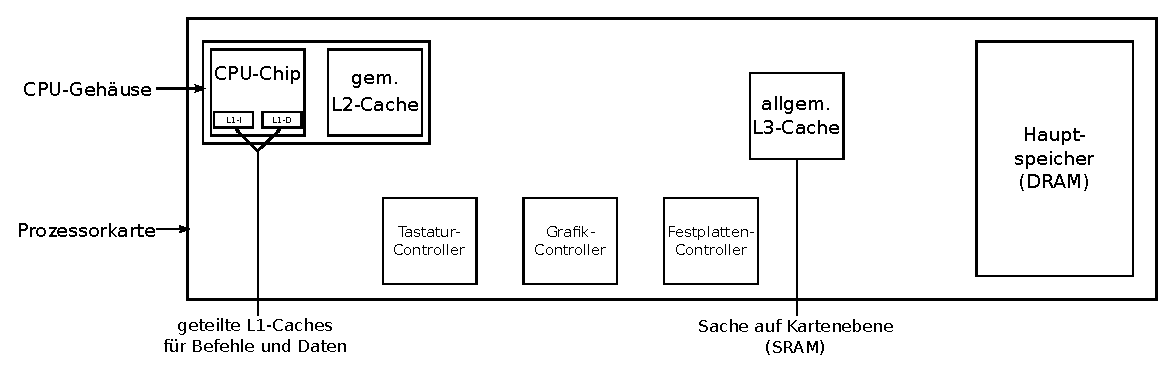
\includegraphics[width=1\textwidth]{Hauptteil/Cache.eps}
\caption{Ein System mit drei Cache-Ebenen nach~\cite{cache}}\label{fig:cache}
\end{figure}





Die Abbildung \ref{fig:cache} zeigt ein klassisches System mit drei Cache-Ebenen. Diese Ebenen unterscheiden sich vorwiegend durch ihre Größe. So beinhaltet der \ac{cpu}-Cache einen kleinen Cache
in der Größenordnung von 16KB bis 64KB. Der Level-2-Cache, welcher neben dem \ac{cpu}-Chip angeordnet und mit einem Hochgeschwindigkeitspfad verbunden ist, besitzt üblicherweise eine Größe von
 512 KB bis 1 MB. Hierbei handelt es sich typischerweise um einen sogenannten \emph{unified} (gemeinsamen) Cache, welcher eine Mischung aus Daten und Befehlen beinhaltet. \\
 Die dritte Cache-Ebene besteht aus einigen Megabyte \ac{sram} und wird auf der Prozessorkarte angeordnet. Dieser \ac{sram} bietet einen enormen Vorteil in der Geschwindigkeit gegenüber dem
 Hauptspeicher(\ac{dram}). \\
 Eine Besonderheit der Caches ist, dass diese umfassend sind, das bedeutet, dass der gesamte Inhalt des L1-Caches im L2-Cache und der gesamte L2-Cache Inhalt im L3-Cache  enthalten ist.\\
 \newpage
Bei dem Prinzip der Adresslokalitäten bedienen sich Caches zwei verschiedenen Arten:\\

\begin{itemize}
  \item örtliche Lokalität (Spartial Locality): Beschreibt die Beobachtung, dass auf Speicherstellen mit 	Adressen, die einer kürzlich angesprochenen Speicherstelle numerisch ähnlich sind, in der
   	nächsten Zeit wahrscheinlich zugegriffen wird. Dadurch werden mehr Daten eingelesen als 	angefordert und damit die Annahme getätigt, dass Anforderungen vorausgesagt werden 	können.
  \item zeitliche Lokalität (Temporal Locality): Auf Speicherstellen, auf die kürzlich zugegriffen wurde, 	wird erneut zugegriffen.  Als praktisches Beispiel gelten hier Funktionen innerhalb
        einer Schleife. Diese Art der Lokalität wird oft zur Fehlerbehebung genutzt,  wenn es zu Cache-	Zugriffsfehlern kommt.\\
\end{itemize}

Grundsätzlich basieren Caches auf dem Prinzip, dass der Hauptspeicher in Blöcke unterteilt wird, welche eine feste Größe besitzen. Dies sind die sogenannten Cache-Zeilen (Cache-Lines).
Diese bestehen aus aufeinander folgenden Bytes in einer Größenordnung von 4 bis 64 Bytes. Bei Speicherzugriffen wird geprüft, ob sich das angeforderte Wort im Cache befindet und direkt
vom Prozessor verwendet werden kann. Ist dies nicht der Fall, wird ein Zeileneintrag aus dem Cache entfernt und die benötigte Zeile aus dem Hauptspeicher geladen. \\
Es gibt zwei grundlegende Arten des Caches. Die einfachste Art Cache zu realisieren, ist die Form des direkt abbildenden Caches. Dabei kann jeder Eintrag, beziehungsweise Zeile, genau
eine Cache-Zeile aus dem Hauptspeicher aufnehmen. Besitzt der Cache eine Zeilengröße von 32 Bytes, nimmt der Cache 64 KB auf. Daraus lässt sich schlussfolgern, dass eine bestimmtes
Wort an genau einer Stelle im Cache liegen kann. Ist das Wort nicht an dieser Adresse zu finden, ist es auch nicht im Cache enthalten. \\

Diese Adresse lässt sich in vier Komponenten zerlegen:
\begin{itemize}
  \item TAG\@: Entspricht den Tag-Bits, welche in einem Cache-Eintrag gespeichert sind
  \item LINE\@: Beinhaltet die Information, in welchem Cache-Eintrag sich die Daten befinden, falls vorhanden
  \item WORD\@: Gibt an, welches Wort innerhalb einer Zeile angefordert wurde
  \item BYTE\@: Wird in Ausnahmefällen genutzt, um einzelne Bytes anzufordern
\end{itemize}





Mit diesen Eigenschaften stellen die direkt abbildenden Caches den am häufigsten verwendeten Cache-Typen dar, weil diese effektiv arbeiten und Kollisionen, bei zum Beispiel identischer LINE,
selten, beziehungsweise gar nicht vorkommen. \\
Das Problem der Speicherkollisionen lässt sich wiederum mit der Verwendung von zwei oder mehr Zeilen pro Cache-Eintrag lösen. Dieser Typ mit \emph{n}-möglichen Einträgen für jede Adresse,
 wird als n-fach mengen-assoziativen Caches (engl. N-way set-associativ Cache) bezeichnet.Im Vergleich zu dem beschriebenden direkt abbildenden Cache ist der mengen-assoziative Cache
 komplizierter, da sich zwar der korrekte Cache-Ebene aus der Speicheradresse berechnen lässt, hierfür jedoch \emph{n} Einträge geprüft werden müssen. Somit ergibt sich ein Nachteil
 was Schnelligkeit anbelangt, jedoch zeigt die Erfahrung, dass sich der Mehraufwand lohnt und 2-, sowie 4-fach Caches gute Leistungen erzielen können.~\cite{cache} \\


 \section{Peripherie}\label{kap:peripherie}
 Ein Peripheriegerät kann einer Hardware hinzugefügt werden, um die Fähigkeiten zu erweitern. Diese Geräte sind optional und dienen zur Ein- und Ausgabe von Daten.

\subsection{UART}\label{kap:uart}

Um mit Peripheriegeräten zu kommunizieren, kann \ac{uart} als serielle Schnittstelle genutzt werden.
Bei dieser Art der Kommunikation werden serielle Daten zwischen dem Board (\emph{Master})
und dem Empfänger (\emph{Slave}) ausgetauscht. \\
Dabei spielen die TxD und die RxD-Datenleitungen
eine wichtige Rolle, da der Datenaustausch über diese Leitungen realisiert wird.\\
Im Gegensatz, zum Beispiel, zu einer \ac{spi}-Schnittstelle, wird kein Clock-Signal
übertragen um Daten zu validieren. Des Weiteren wird die Verbindung mit einer definierten
Geschwindigkeit realisiert, der sogenannten \emph{Baudrate}. \cite{uartpdf} \\
Die Baudrate bezeichnet dabei die Anzahl der Bits, welche pro Sekunde übertragen werden.
\ac{uart} konvertiert die Bytes in serielle Bits, überträgt diese über eine einzelne Leitung
und liest die zugehörigen Start- und Stop-Bits aus.\\
Das sogenannte \emph{Character}(Zeichen) besteht aus einer konfigurierbaren Anzahl an Datenbits (in den meisten
Fällen 7 oder 8), aus einem \emph{low-level} Start-Bit, einem optionalen Parity-Bit und einem
oder mehreren logischen \emph{high-level} Stop-Bits.\\
Das Start-Bit teilt dem Receiver mit, dass ein neues \emph{Character} empfangen wird.
Die nächsten Bits, je nachdem wie viele Daten-Bits vorher konfiguriert wurden , stellen
dann den Inhalt des \emph{Character} dar. Darauf folgt das optionale Parity-Bit,
welches anzeigt, ob die Anzahl der mit '\emph{1}' belegten Daten-Bits gerade oder
ungerade ist. Am Ende der Folge stehen dann entweder ein oder zwei  \emph{high-level } Stop-Bits,
welche dem Receiver eindeutig signalisieren, dass die Übertragung vollständig ist. Dadurch,
dass das Start-Bit \emph{high-level} (1) und das Stop-Bit \emph{low-level} (0) ist,
ist immer eine klare Abgrenzung zwischen dem derzeitigen und dem folgenden \emph{Character} möglich.\\

Die Datenübertragung lässt sich nach~\ref{fig:uart} darstellen.\\

\begin{figure}[h!]
\centering
\includegraphics[width=0.8\textwidth]{Hauptteil/uart.eps}
\caption{Datenübertragung per \ac{uart}(8n1) }
\label{fig:uart}
\end{figure}


\subsection{Interrupt}\label{kap:interrupt}
Neben der \ac{cpu} und dem Datenspeicher haben die meisten Computersysteme Peripherie. Es handelt sich dabei um verbaute oder um an Schnittstellen angeschlossene Geräte.
Damit die \ac{cpu} die Nachricht erhält, dass Daten an solch einer Schnittstelle beziehungsweise Verbindung anliegen, muss es eine Möglichkeit geben den Prozessor zu
unterbrechen. Hier gibt es die Art des sogenannten Polling, bei dem der Prozessor alle vorhandenen Eingabegeräte zyklisch abfragt. Ein effektiveres Verfahren ist die
Unterbrechungsanforderung (Interrupt), welche eintritt, wenn Daten anliegen. \\
Sobald ein Gerät Daten zur Weiterverarbeitung besitzt, wird ein \ac{irq} auf der dafür vorgesehenen Interrupt-Leitung gesendet. Daraufhin unterbricht der Prozessor
seine Arbeit und verarbeitet die Daten des Gerätes.\cite{irq}\\

\begin{figure}[H]
\centering
\includegraphics[width=0.8\textwidth]{Hauptteil/irq.eps}
\caption{Interrupt-Controller}\label{fig:irq}
\end{figure}

\subsection{Timer}\label{kap:timer}

Ein weiterer essenzieller Teil zur Ausführung eines Betriebssystems, wie zum Beispiel Linux, ist der Timer. Dieser hilft dem Betriebssystem dabei, das so genannte Scheduling
durchzuführen. Hierbei wird mit Hilfe von \emph{Timer}-gesteuerten Interrupts dafür gesorgt, dass Nutzerprogramme, welche sich in der Ausführung befinden, unterbrochen werden und
in den Betriebssystem-Modus geschaltet wird. Nun kann das Betriebssystem die anstehenden Prozesse neu planen.\\


\section{Compiler}\label{kap:compiler}

Der Compiler ist ein Werkzeug, welches einen Quelltext, der in einer höheren Programmiersprache (C++, C, Java) geschrieben wurde, in Maschinenbefehle umsetzt.
 Damit der Prozessor diese Instruktionen ausführen kann, werden die lesbaren Programmierbefehle übersetzt. Nach dem so genannten Kompilieren steht das Programm zur Ausführung bereit.
Die Aufgaben des Compilers bestehen grundsätzlich aus drei Schritten:\cite{compiler}
\begin{enumerate}
  \item Lexikalische Analyse:
  	Der Compiler zerlegt die Wörter und Zeichen des Quelltextes in verschiedene Klassen. Dabei werden überflüssige oder fehlende Zeichen als Fehler erkannt und vom Compiler, je nach
  schwere des Verstoßes, als Warning oder Error ausgegeben.
  \item Parsing:
  	Es folgt die Prüfung des Codes auf syntaktische Korrektheit.
  \item Semantische Analyse: Der Quelltext wird auf Sinnhaftigkeit geprüft. Zum Beispiel ob Befehle wirklich die korrekten Parameter haben.
\end{enumerate}

Im Vergleich zum Interpreter gibt es folgende Vor- und Nachteile.

Vorteile:
\begin{itemize}
  \item effiziente Übersetzung in ausführbaren Code
  \item Optimierung des generierten Codes
\end{itemize}

Nachteile:
\begin{itemize}
  \item Kompilieren benötigt Zeit und Ressourcen
  \item Neu-Kompilierung nach Quelltextänderung
  \item Jede Programmiersprache benötigt einen eigenen Compiler
\end{itemize}

\begin{figure}[H]
\centering
\includegraphics[width=0.8\textwidth]{Hauptteil/Compiler.eps}
\caption{Funktionsweise des Compilers}\label{fig:compiler}
\end{figure}

\subsection{Compiler-Modi}\label{kap:compilermode}

Der im Kapitel zuvor beschriebene Compiler kann, je nach Zielsystem, in verschiedenen Modi betrieben werden. Hier bei ist der ausschlaggebende Punkt, ob auf dem System ein Betriebssystem ausgeführt werden soll oder nicht.\\

\begin{itemize}
  \item Non-OS mode: Programme ohne Zugriff auf Ein- bzw. Ausgabegeräte. Programme, welche in diesem Modus ausgeführt werden, haben keine periphere Unterstützung.
        Der Bare-Metal-Mode wird meistens genutzt, um \ac{isa}- und Cache-Regressionstests durchzuführen. Hierbei entscheidet der Rückgabewert des Programmes über Erfolg beziehungsweise Misserfolg
        des Tests. \emph{0} bedeutet Erfolg, Zahlen ungleich \emph{0} geben den jeweiligen Fehlercode an. Bare-Metal-kompilierte Programm laufen auf einem \ac{fpga} und in einer Simulation
        im Hintergrund. \\
        Um nun mit einem Bare-Metal-Programm eine Ausgabe zu erzeugen, müssen Bibliothkenen verwendet werden, welche die Art und Weise der Ausgabe beinhalten.\\

        \begin{figure}[H]
        \centering
        \includegraphics[width=0.4\textwidth]{Hauptteil/baremetal.eps}
        \caption{Grafische Darstellung der Non-OS-Architektur}\label{fig:baremetal}
        \end{figure}

  \item Linux mode: Benutzerprogramme mit Linux-Unterstützung. Mit Hilfe dieser Programme lassen sich Verhaltssimulationen auf dem \ac{fpga}-Board durchführen. Diese Programme
  erhalten Multi-Thread und Peripherie-Unterstützung vom Linux-Kernel\cite{lowrisc}\\

  \begin{figure}[H]
  \centering
  \includegraphics[width=0.4\textwidth]{Hauptteil/linuxmode.eps}
  \caption{Grafische Darstellung der Linux-Architektur}\label{fig:linuxmode}
  \end{figure}
\end{itemize}




\section{Linux}\label{kap:linux}


Das verwendete System Linux wurde als freies Betriebssystem von Linus Benedict Torvald entwickelt.
Es basiert auf dem Unix-Modell, jedoch schrieb Torvald den sogenannten Kernel neu. Seit dem gilt
Linux als Open-Source-Projekt und Entwickler versuchen stetig das System zu verbessern.\cite{linux}\\
Die wohl wichtigste Eigenschaft die Linux bzw. Unix für den Einsatz beliebt macht, ist die Portabilität,
da es weitestgehend rechnerunabhängig läuft. Weitere Eigenschaften die das Betriebssystem zu einem der
 weitverbreitetsten Systeme überhaupt gemacht haben, sind:\\\cite{linux}\\
\begin{itemize}
\item  \textbf{Multi-Tasking} Das parallele Nutzen verschiedener Programme erlaubt jedem Benutzer
        gleichzeitige Aktionen durchzuführen, ohne auf den Abschluss der letzten Tätigkeit zu warten.
\item  \textbf{Time-Sharing} Das Priorisieren von einzelnen Prozessen erlaubt es, dass mehrere
        Prozesse gleichzeitig ablaufen, indem abwechselnd Platz im Hauptspeicher beziehungsweise in der \ac{cpu}
        zugewiesen wird.
\item \textbf{Sprachenvielfalt} Neben der Sprache C stellt Linux/Unix viele Programmiersprachen
      wie C++, Java, Python und viele mehr zur Verfügung. Dadurch, dass es sich um ein Open-Source-Projekt handelt,
      wird diese Bibliothek, je nach System, ständig erweitert.
\item \textbf{Grafische Benutzeroberfläche} Linuxrechner, im speziellen die Anwendungen, nutzen in
      den meisten Fällen \ac{gnome} oder \ac{kde} als grafische Oberfläche. Durch die weitverbreitete Nutzung
      dieser Oberflächen wurden diese kontinuierlich weiterentwickelt und bieten so eine hohe Vielfalt an
      Anpassungsmöglichkeiten.
\item \textbf{Netzwerk} Für die Kommunikation zwischen Server und Client hat sich das Betriebssystem bewährt,
      da es über ein umfangreiches Paket an Software verfügt. Neben den Standardprotokollen \ac{tcpip} (IPv6 wird
      ebenfalls unterstützt), werden weitere Formate verwendet, wie zum Beispiel \ac{uucp}, welches eine simple Form
      der Kommunikation zwischen Linux/Unix-Rechnern darstellt.
\end{itemize}

Grundsätzliche bestehen Betriebssysteme wie Linux/Unix aus drei Hauptkomponenten.
Der \textbf{Kern} (engl. \emph{Kernel}) bildet die grundlegenden Funktionen, wie
zum Beispiel die Organisation und Verwaltung von Speicher, der Prozesse, sowie
Ein- und Ausgänge und sämtliche Kommunikationsaufgaben.\\
Das \textbf{Dateisystem} (engl. \emph{File System}) ermöglicht das Speichern von Dateien
und errichtet einen Dateibaum und ist somit für die Datenorganisation zuständig.\\
Die dritte Komponente stellt der \textbf{Befehlsübersetzer} dar (engl. \emph{shell}),
welcher anhand einer Befehlssprache die Kommunikation ermöglicht und dem Benutzer erlaubt
mit sämtlichen Peripheriegeräten zu interagieren, ohne dass die im Hintergrund laufenden
Prozesse berücksichtigt werden müssen. \cite{ubuntu}\\

Grafisch lässt sich der Aufbau wie folgt darstellen:\\

\begin{figure}[H]
\centering
\includegraphics[width=0.55\textwidth]{Hauptteil/csa.eps}
\caption{Computer System Architektur nach \cite{virtualmachines}}
\label{fig:mbs}
\end{figure}

Um nun mit den verschiedenen Geräten über eine Vielzahl von Schnittstellen kommunizieren
zu können, benötigt jedes Gerät einen eigenen Treiber. Dieser Treiber ist im Betriebssystem
als \emph{„Wissen“} hinterlegt und beinhaltet Information über das Gerät und dessen
Zugriffsmöglichkeiten und wird im folgenden Unterkapitel näher erklärt. \cite{treiber}\\
Der Anwender hat nun die Möglichkeit über die Treiber auf die Schnittstellen zuzugreifen, in dem diese vom
Treiber gesteuert werden.

\subsection{Treiber}\label{kap:treiber}

Der Treiber gilt als \emph{„Lexikon“} der jeweiligen Geräte für das Betriebssystem.
Diese Aufgabe ist enorm wichtig für ein funktionierendes System, sodass der Stellenwert
eines Treibers sehr hoch ist. Einfach erklärt, besteht ein Treiber aus einer Reihe von
Funktionen, die den Zugriff auf das Gerät steuern und so eine Kommunikation ermöglichen.
So muss für jedes Gerät ein eigener Treiber implementiert werden, der die offene
Schnittstelle im Betriebssystemkern füllt. \\
Dabei sind zwei Begrifflichkeiten wichtig, in die der Speicherbereich aufgeteilt wird:
\begin{itemize}
\item \textbf{Kernelspace} : Diese Bereich wird ausschließlich vom Kernel benutzt
\item \textbf{Userspace} : Dieser Speicher wird von Applikationen genutzt und kann nicht,
                          oder in Ausnahmfällen, nur eingeschränkt vom Kernel genutzt werden
\end{itemize}

Die Treiber werden grundsätzlich mit in den Kernel kompiliert oder sind als Modul dynamisch
angelegt, um zum Kernel, während der Laufzeit, hinzugefügt zu werden. \cite{treiberbib}\\

Bei der Implementierung von Gerätetreibern wird zwischen drei Gerätetypen unterschieden (\cite{treiberbib}):\\
\begin{enumerate}
\item \textbf{Character-Devices} Auf diese Geräte kann wie auf einen Stream von Bytes zugegriffen werden, indem
      \ac{posix}-Funktionen genutzt werden, wie beispielsweise \emph{open()},\emph{write()},\emph{read()} oder \emph{close()}.
      Für die Nutzung wird für jedes Gerät eine \emph{Gerätedatei} (vgl. \emph{device nodes}) angelegt.
\item \textbf{Block Devices} Im Gegensatz zu den \emph{Character-Devices}, wird auf die \emph{Block-Devices} immer per Random Access zugegriffen.
      Die Daten werden blockweise gelesen. Diese \emph{Block-Devices} können ein Dateisystem aufnehmen und gemountet werden.
\item \textbf{Netzwerkschnittstellen} Netzwerkgeräte erhalten keine Gerätedatei, sondern sind in einer globalen Liste hinterlegt.
      Der Datenaustausch findet immer asynchron statt, sodass die Netzwerkkarte jederzeit bereit sein muss Daten zu empfangen.
\end{enumerate}

%
% \subsection{Device Tree}\label{kap:devicetree}
%
%
% Der \emph{Device-Tree} beinhaltet
% Informationen, welche dem Kernel bei dem Bootvorgang helfen. Da das System angeschlossene Geräte nicht automatisch erkennen
% und die dazu passenden Treiber laden kann, geschieht das in dieser \emph{.dts}-Datei. Durch das Kompilieren wird daraus
% der sogennante \emph{Device} \emph{Tree} \emph{Blob}. Dieser wird zusammen mit dem Kernel vom Bootloader geladen und im
% Hauptspeicher abgelegt. Im Anschluss daran wird daraus eine Baumstruktur. In dieser sind die Geräte als Knoten angelegt
% und es werden Informationen zu den dazugehörigen Treiber hinterlegt, welche dem Betriebssystem zur Verfügung gestellt werden.
% Die Verbindung zwischen Device-Tree und dem Treiber wird über eine
% eindeutige Identifikation per \emph{Compatible} festgelegt.
%
%
% \subsection{Buildroot}\label{kap:buildroot}
%
% \emph{Buildroot} ist ein Tool, welches das Erstellen eines kompletten Linux-Systems per
% \emph{Cross-Compiling} für eingebettete Systeme vereinfacht und automatisiert.  Neben dem
% \emph{cross-compiled} Toolchain können ebenfalls das \emph{Root}-Dateisystem, ein \emph{Linux-Kernel-Image}
% und ein \emph{Bootloader} für das Zielsystem erstellt werden.  In einem Konfigurationsprogramm lassen sich vor der
% Erstellung sämtliche Optionen und Erweiterungen ab- beziehungsweise anwählen. \\
% Das Tool wird größtenteils dafür genutzt, um die Systeme für andere Prozessoren, außer die klassischen x86-Prozessoren,
% zu erstellen, wie zum Beispiel \ac{arm}-Prozessoren.\cite{buildroot}\\
%
% \textbf{Toolchain}\\
%
% Bei der \emph{Toolchain} handelt es sich um eine Reihe von Tools zum Erstellen und Debuggen von Code für eine Zielarchitektur. Des Weiteren beinhaltet sie einen Compiler, einen Linker,
%  sowie verschiedene Bibliotheken.\\
%  Die Toolchain ist essenziell, um die drei weiteren Elemente eines eingebetteten Systems zu generieren: den Bootloader, den Kernel und das Root-Dateisystem. \\
%  Hierbei wird im wesentlichen zwischen zwei \emph{Toolchain}-Arten differenziert:
%  \begin{enumerate}
%    \item Die interne Toolchain: Die \emph{Toolchain} wird aus einer Quelle heraus vom \emph{Buildroot} generiert
%    \item die externe Toolchain: Es wird eine bereits vorhandene \emph{Toolchain} verwendet
%  \end{enumerate}
%
% Das Generieren einer eigenen \emph{Toolchain} benötigt entsprechend mehr Zeit und verlängert den ganzen Kompiliervorgang, bietet jedoch deutlich mehr Konfigurationsmöglichkeiten
% im Vergleich zu bereits vorhandenen \emph{Toolchains}.\\
%
% \textbf{Kernel}\\
%
% Der \emph{Kernel}, welcher bereits in Kapitel~\ref{kap:linux} beschrieben wurde, kann ebenfalls durch \emph{Buildroot} konfiguriert und erzeugt werden.\\
% Dieser steuert alle Prozessor-und Speicherzugriffe, unterhält die wichtigsten Treiber und greift direkt auf die Hardware zu. Dadurch, dass er die unterste Schicht des Systems beschreibt,
% ist er die Basis in der Kommunikation zwischen Hard- und Software.\\
% Zu seinen Aufgaben gehören neben der parallelen Verarbeitung verschiedener Aufgaben, auch die Einhaltung zeitkritischer Grenzen, sowie die Offenheit für unterschiedlichste Anwendungen
% und Erweiterungen. Im Falle des Linux-Systems gilt der Kernel als Vermittler im System, so ist die grafische Oberfläche komplett unabhängig vom Linux-Kernel.\cite{datacenter}\\
%
% \textbf{Root-Dateisystem}\\
%
% Der Kernel enthält keine Programme oder Dämonen, die das System an sich nutzbar machen. Hierfür ist das \emph{Root-Dateisystem} zuständig.\\
% Wichtige Inhalte sind:
% \begin{itemize}
%   \item init-Dämon: Startet Dämonen, Systemeinstellungen sowie Login-Programme
%   \item System-Konfiguration
%   \item Device-Nodes
%   \item Bibliotheken und Kernel-Module
% \end{itemize}
%
% Für die Zusammenstellung dieses Dateisystem kann \emph{Buildroot} verwendet werden, wodurch \emph{BusyBox} sowie weitere Programmpakete integriert werden.\cite{elektronikpraxis}\\
%
% \textbf{Bootloader}\\
%
% Der Bootloader, auch Boot Manager genannt, ist ein Programm, dessen Aufgabe es ist, das Betriebssystem in den Arbeitsspeicher zu laden. In diesem Fall ist er dafür verantwortlich,
% den Kernel mit den gewünschten Parametern zu laden und den Speicher zu initialisieren, bevor der eigentliche Boot-Prozess startet.\cite{searchdatacenter}\\
%
% \textbf{BusyBox}\\
%
% BusyBox kombiniert winzige Versionen vieler gängiger UNIX-Dienstprogramme in einer einzigen kleinen ausführbaren Datei.
% Es bietet Ersatz für die meisten Dienstprogramme, die normalerweise in GNU fileutils, Shellutils zu finden sind.
% Die Dienstprogramme in BusyBox haben im Allgemeinen weniger Optionen als ihre voll ausgestatteten GNU-Gegenstücke, welche jedoch die erwartete Funktionalität bieten und vom Verhalten sehr ähnlich sind.
% Ebenfalls bietet die BusyBox eine ziemlich vollständige Umgebung für eingebettete Systeme.\\
% BusyBox wurde größenoptimiert und für begrenzte Ressourcen geschrieben.
% Es ist auch extrem modular, sodass Befehle (oder Funktionen) zur Kompilierzeit ein- und ausgeschlossen werden können.
% Dies erleichtert die schnelle Anpassung der eingebetteten Systeme.\cite{busybox}\\
%

\chapter{Soft Cores}\label{kap:softcores}
\section{MicroBlaze basierte Systeme}\label{kap:microblaze}
Microblaze

Der MicroBlaze SoftCore von Xilinx ist eine 32-Bit RISC Harvard Architektur mit einem umfangreichen Befehlssatz und ist optimiert für eingebettete Anwendungen.
Neben dieser Flexibilität besitzt er drei unterschiedliche Voreinstellungen:

\begin{enumerate}
  \item Microcontroller: Geeignet für Baremetall-Code
        \begin{itemize}
          \item 32-Bit Prozessorkern (in der Regel ohne \ac{mmu})
          \item Externer Speichercontroller
          \item \ac{spi} Controller
          \item I2C-Controller
          \item \ac{uart}
          \item Interrupt-Controller
          \item  Timer
        \end{itemize}
  \item Echtzeitprozessor: Deterministische Echtzeitverarbeitung auf einem \ac{rtos}
    \begin{itemize}
      \item Alle Mikrocontroller Blöcke
      \item Instruktioncache
      \item \ac{mpu}
      \item Datencache
      \item DDR-Controller
      \end{itemize}
  \item Anwendungsprozessor: Embedded Linux-fähig
        \begin{itemize}
          \item Alle Echtzeit-Prozessor-Blöcke
          \item 32-Bit-Prozessorkern
          \item \ac{mmu}
          \item Ethernet-Controller
        \end{itemize}
\end{enumerate}

Ausgehend von diesen Presets lässt sich das Design mit Hilfe von spezifischen Prozessoroptionen anpassen.
 Diese Vielanzahl an Anpassungen sind per Drag \& Drop sehr einfach hinzuzufügen. Dazu zählen unter anderem \ac{uart}-,\ac{pwm}- und \ac{dma}-Bausteine, sowie serielle Schnittstellen.
 Dadurch wird sichergestellt, dass die spezifischen Anforderungen der Anwendung erfüllt werden.

Zusammengefasst besitzt der Microblaze folgende Schlüsselfähigkeiten:
\begin{itemize}
  \item 32 mal 32-Bit-\emph{General-Purpose}-Register
  \item 32-Bit-Befehlswort mit drei Operanden und zwei Adressierungsmodi
  \item 32-Bit-Adressbus, erweiterbar auf 64-Bit
  \item Optionale \ac{fpu}
  \item \ac{axi}4-Interface
  \item Verschiedene Zustandsmodi (Sleep, Hibernate, Suspend Mode/Instrctions)
  \item Unterstützt entweder \ac{plb}- oder \ac{axi}-Schnittstellen
  \item Big-Endian / Little-endian Unterstützung
  \item Optionale \ac{mmu}, sowie separate, konfigurierbare Daten- und Instruktionscaches
\end{itemize}


\newpage
\section{lowRISC basierte Systeme}\label{kap:lowrisc}


\section{LEON3 basierte Systeme}\label{kap:leon3}

Der LEON3 ist das \ac{vhdl}-Modell eines 32-Bit-Prozessors, welcher auf der SPARC V8-Architektur basiert. Das Modell ist in großem Umfang konfigurierbar und besonders für \ac{soc}-Designs geeignet.
Ursprünglich wurde dieses System von der \ac{esa} entworfen, wird heutzutage jedoch von \emph{Aeroflex Gaisler} weiterentwickelt und vertrieben.\\
Der LEON3-Prozessor verfügt über folgende Eigenschaften:\cite{leon}\\

\begin{itemize}
  \item SPARC V8 Befehlssatz mit V8e Erweiterungen
\item Fortgeschrittene 7-stufige Pipeline
\item Hardware multiplizieren, teilen und \ac{mac}-Einheiten
\item Hochperformante IEEE-754-\ac{fpu} mit vollem Pipelinespektrum
\item Getrennter Befehls- und Datencache (Harvard-Architektur) mit Snooping
\item Konfigurierbare Caches: 1 - 4 Wege, 1 - 256 kbytes / Weg. Random,LRR oder \ac{lru} Ersatz
\item Lokaler Befehls- und Daten-Scratchpad-RAM, 1 - 512 KByte
\item \ac{srmmu} mit konfigurierbarem \ac{tlb}
\item \ac{amba}-2.0 \ac{ahb}-Busschnittstelle
\item Erweiterte On-Chip-Debug-Unterstützung mit Befehls- und Daten-Trace-Puffer
\item Symmetrische Multiprozessorunterstützung (\ac{smp})
\item Power-Down-Modus und Clock-Gating
\item Robustes und vollsynchrones Single-Edge-Clock-Design
\item Bis zu 125 MHz in FPGA und 400 MHz in 0,13 um \ac{asic}-Technologien
\item Fehlertolerante und SEU-geschützte Version für Raumfahrtanwendungen
\item umfangreich konfigurierbar
\item Große Auswahl an Software-Tools: Compiler, Kernel, Simulatoren und Debug-Monitore
\item Hohe Leistung: 1,4 DMIPS / MHz, 1,8 CoreMark / MHz (gcc -4.1.2)
\end{itemize}
